\chapter{Introducción}

% \defaultFontEpigraph{All You Need Is a Good Init}{\cite{mishkinAllYouNeed2016}}
\defaultFontEpigraph{All You Need Is a Good Init}{Mishkin y Matas (2016)}

\todo[]{Realizar la introducción del trabajo siguiendo estos puntos.}
A realizar:
\begin{itemize}
    \item Presentar el trabajo de forma atractiva
    \begin{itemize}
        \item Traer algunas ideas de Justificación
        \item Explicar título "All You Need" y epígrafes. Nos apoyamos en la Figura \ref{fig:all_you_need_publicaciones}
        \item Este trabajo es investigación, pero tiene como fruto un software de \textit{live coding}, \textit{AI Muse} y una obra de arte sonoro, \textit{AlgorAI}
    \end{itemize}
    \item Describir los deferentes capítulos
    \item Explicar el uso de acrónimos
    \item Explicar la razón del uso de gran parte de los términos de IA en inglés
    \item Explicar el uso de los QR
\end{itemize}




\begin{figure}[H]
    \caption[Número de publicaciones de \textit{Deep Learning} por año que contienen la expresión <<all you need>> en el título]{Número de publicaciones de \textit{Deep Learning} por año que contienen la expresión <<all you need>> en el título.}
    \centering
    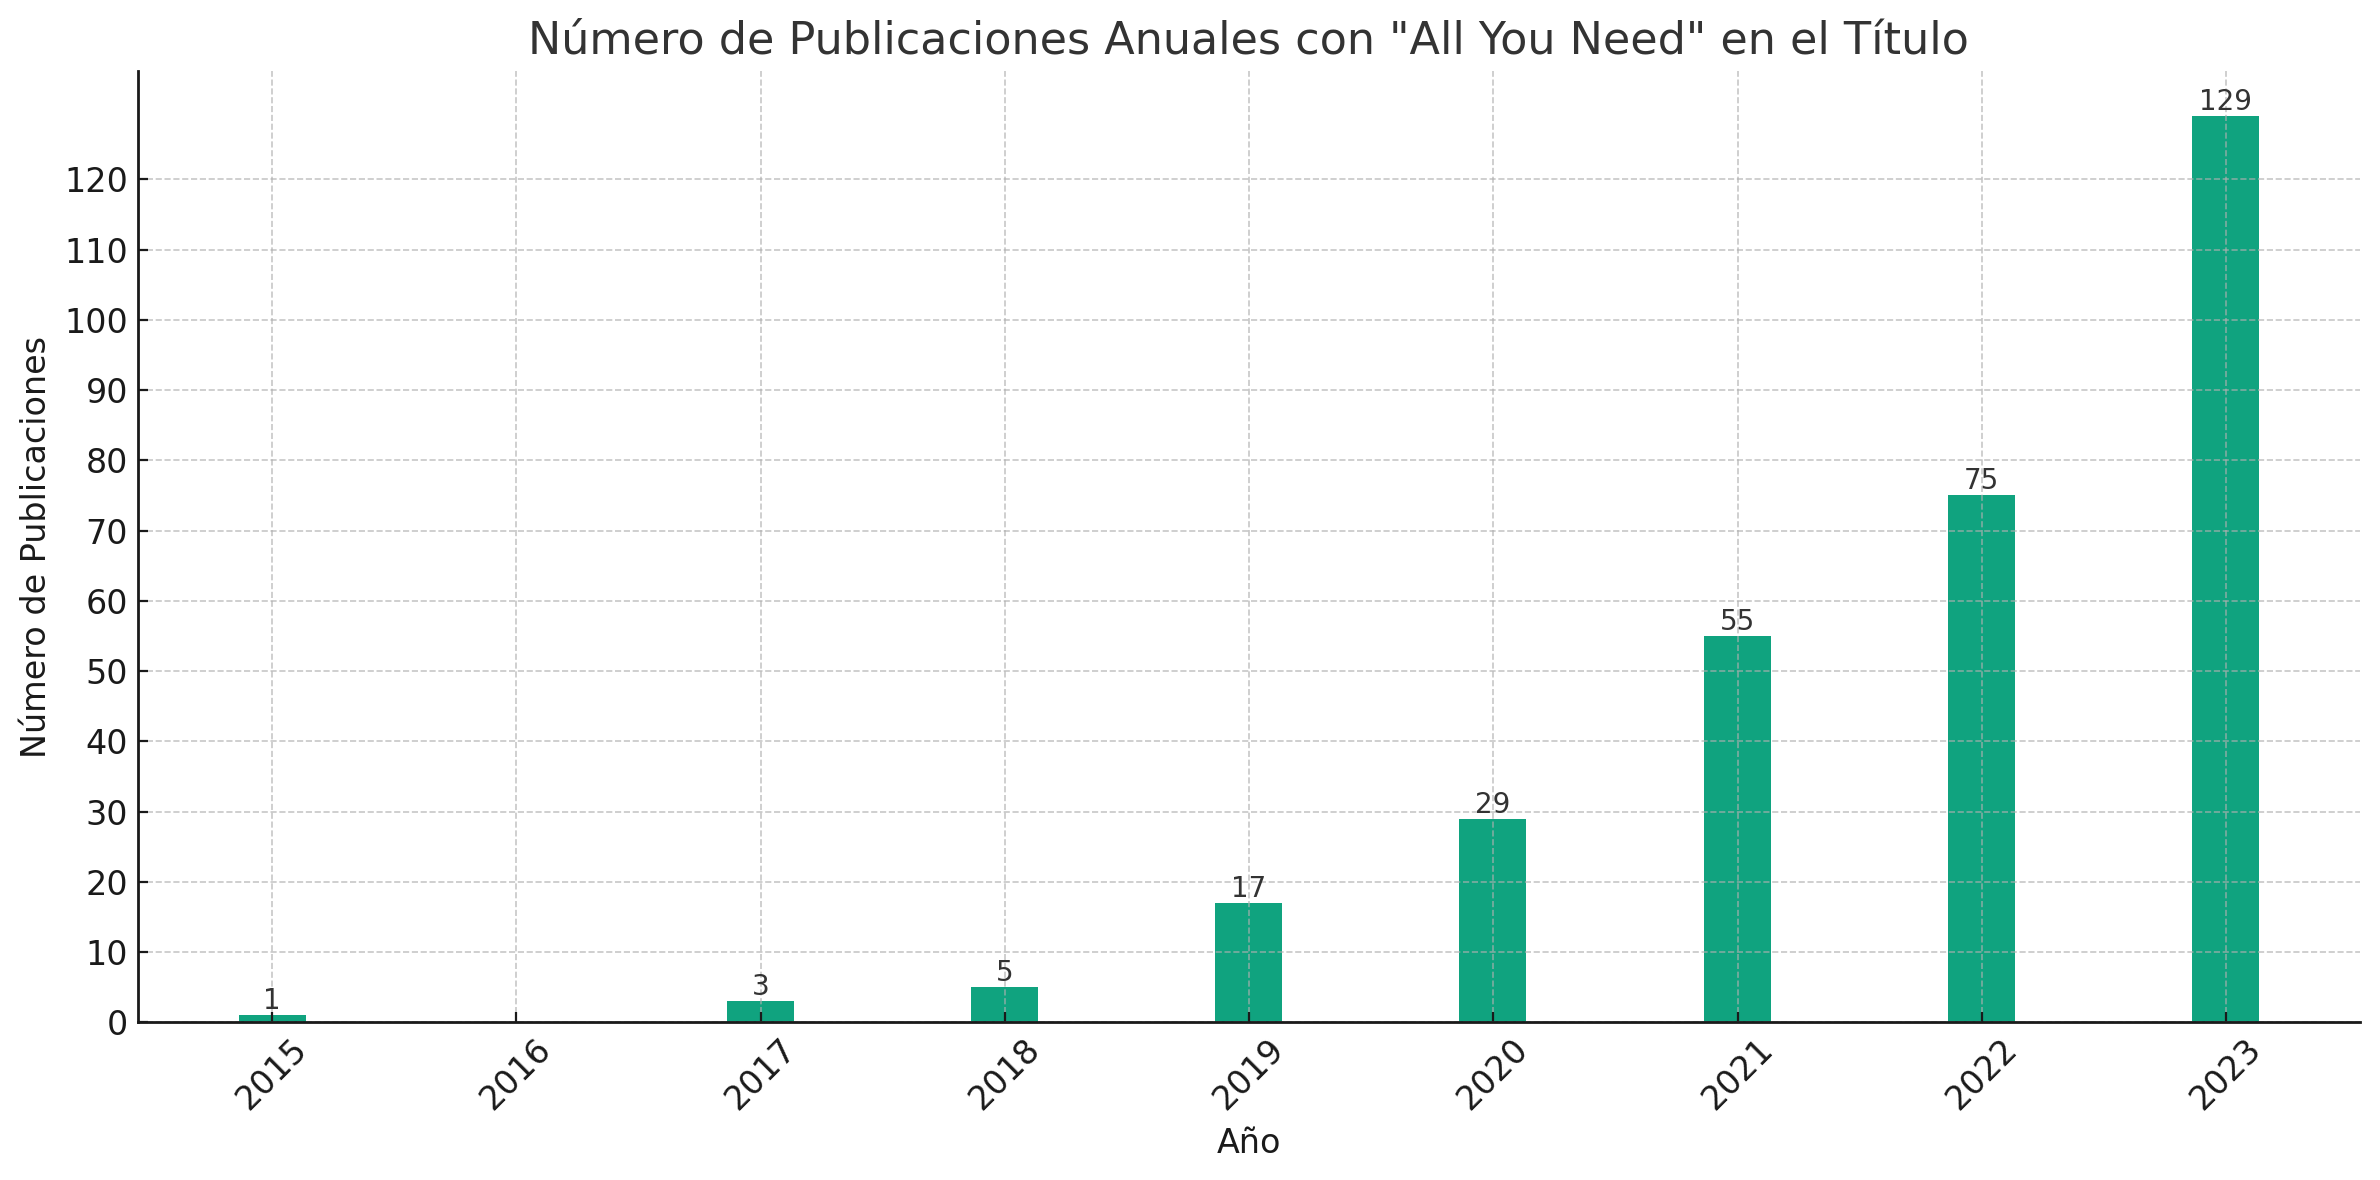
\includegraphics[width=0.9\textwidth]{./figuras/all_you_need_publicacionies_anuales.png}
    \source{Elaboración propia a partir del listado de \url{https://github.com/KentoNishi/awesome-all-you-need-papers}}
    \label{fig:all_you_need_publicaciones}
\end{figure}


Nos encontramos en una era tecnológicamente acelerada donde la investigación se vuelve esencial, a pesar de que pueda quedar obsoleta en un corto período. En unos pocos años, será impensable un ámbito de la vida humana que quede fuera del alcance de la \gls{ia}. Es esperable que todo profesional, incluso en campos artísticos, incorpore estas herramientas en su trabajo. Por otra parte, cualquier retroalimentación al \gls{dl}, por mínima que sea, en este caso desde el ámbito musical, se presenta como necesaria para comprender mejor su funcionamiento.

Queda fuera de este estudio cualquier evaluación ética o antropológica de la \gls{ia}, más allá de una perspectiva práctica y descriptiva del uso de los \gls{llm} en la creación musical y sonora, asumiendo que, al momento de esta investigación, los \gls{llm} pueden razonar y crear a niveles que se acercan al de los humanos. Como toda nueva tecnología, ha de madurar en el colectivo humano y encontrar su lugar de integración en lo laboral, lo artístico, lo ético y lo legal, para así tener una fotografía más amplia de lo que la \gls{ia} significa.



